\documentclass[lang = cn, scheme = chinese, thmcnt = section, usesamecnt]{elegantbook}
% elegantbook      设置elegantbook文档类
% lang = cn        设置中文环境
% scheme = chinese 设置标题为中文
% thmcnt = section 设置计数器


%% 1.封面设置

\title{Galois 理论 - 笔记}                % 文档标题

\author{若水}                        % 作者

\myemail{ethanmxzhou@163.com}       % 邮箱

\homepage{helloethanzhou.github.io} % 主页

\date{\today}                       % 日期

\logo{PiCreatures_happy.pdf}        % 设置Logo

\cover{阿基米德螺旋曲线.pdf}          % 设置封面图片

% 修改标题页的色带
\definecolor{customcolor}{RGB}{135, 206, 250} 
% 定义一个名为customcolor的颜色,RGB颜色值为(135, 206, 250)

\colorlet{coverlinecolor}{customcolor}     % 将coverlinecolor颜色设置为customcolor颜色

%% 2.目录设置
\setcounter{tocdepth}{3}  % 目录深度为3

%% 3.引入宏包
\usepackage[all]{xy}
\usepackage{bbm, svg, graphicx, float, extpfeil, amsmath, amssymb, mathrsfs, mathalpha, hyperref, graphicx, romannum, chemarrow, booktabs, fontspec, ctex, stmaryrd, MnSymbol}

%% 4.定义命令
\newcommand{\N}{\mathbb{N}}            % 自然数集合
\newcommand{\R}{\mathbb{R}}            % 实数集合
\newcommand{\C}{\mathbb{C}}  		   % 复数集合
\newcommand{\Q}{\mathbb{Q}}            % 有理数集合
\newcommand{\Z}{\mathbb{Z}}            % 整数集合
\newcommand{\F}{\mathbb{F}}
\newcommand{\sub}{\subset}             % 包含
\newcommand{\im}{\text{im }}           % 像
\newcommand{\lang}{\langle}            % 左尖括号
\newcommand{\rang}{\rangle}            % 右尖括号
\newcommand{\dis}{\displaystyle}
\newcommand{\cont}{\mathrm{cont}}
\newcommand{\cha}{\mathrm{char}}
\newcommand{\Gal}{\mathrm{Gal}}
\newcommand{\Aut}{\mathrm{Aut}}
\newcommand{\Inv}{\mathrm{Inv}}
\newcommand{\function}[5]{
\begin{align*}
	#1:\begin{aligned}[t]
		#2 &\longrightarrow #3\\
		#4 &\longmapsto #5
	\end{aligned}
\end{align*}
}                                     % 函数

\newcommand{\lhdneq}{%
\mathrel{\ooalign{$\lneq$\cr\raise.22ex\hbox{$\lhd$}\cr}}} % 真正规子群

\newcommand{\rhdneq}{%
\mathrel{\ooalign{$\gneq$\cr\raise.22ex\hbox{$\rhd$}\cr}}} % 真正规子群

\newcommand{\upiff}{\mathrel{\rotatebox[origin=c]{90}{$\iff$}}} % 竖着的等价

\newcommand{\Rmnum}[1]{\uppercase\expandafter{\romannumeral #1}}  %定义命令输入大写罗马数字
\newcommand{\rmnum}[1]{\romannumeral #1}  %定义命令输入小写罗马数字

\newcommand{\testleftlong}{\longleftarrow\mkern-7.5mu\shortmid}

\begin{document}

\maketitle       % 创建标题页

\frontmatter     % 开始前言部分

\begin{figure}[p]
	\centering
	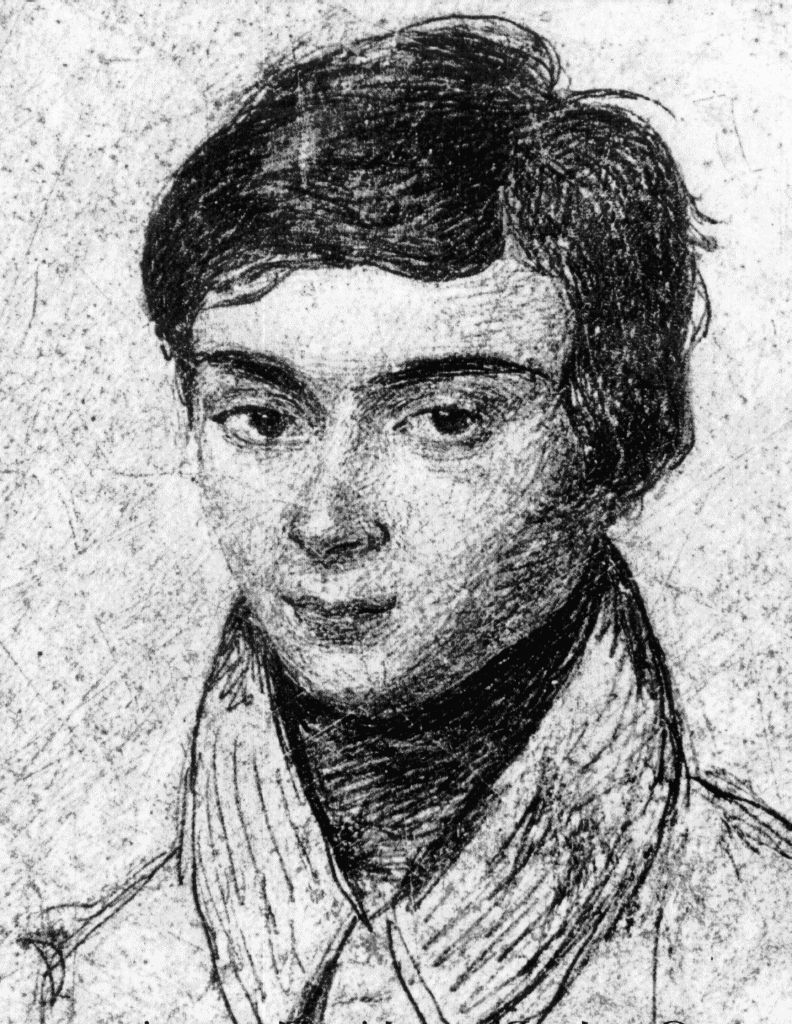
\includegraphics[width=0.5\textwidth]{../figure/Evariste Galois}
	\vspace{2.1cm}
	
	{\large\fontspec{EB Garamond} Après cela, il y aura, j'espère, des gens qui trouveront leur profit à déchiffrer tout ce gâchis.}
	
	\begin{flushright}
		--- {\large\fontspec{EB Garamond} Evariste Galois}
	\end{flushright}
\end{figure}

\tableofcontents % 创建目录

\mainmatter      % 开始正文部分

\chapter{Galois扩张}

\section{Galois对应}

\begin{definition}{域扩张}
	对于域$k$与$K$,称$K/k$为域扩张,如果存在同态映射$\varphi:k\to K$。
\end{definition}

\begin{definition}{中间域}
	对于域扩张$k\sub F \sub K$,称$F$为$K/k$的中间域。
\end{definition}

\begin{definition}{自同构群}{自同构群}
	定义域$K$的自同构群为
	$$
	\Aut(K)=\{ \text{同构映射}\varphi:K\to K \}
	$$
\end{definition}

\begin{definition}{$k$-自同构群}{k-自同构群}
	定义域扩张$K/k$的$k$-自同构群为
	$$
	\Aut_k(K)=\{ \text{同构映射}\varphi:K\to K\mid \varphi(x)=x,\forall x\in k \}
	$$
\end{definition}

\begin{proof}
	我们来证明$\Aut_k(K)$关于映射的复合构成群。
	
	对于封闭性,任取$\varphi,\psi\in \Aut_k(K)$,由于$\varphi,\psi:K\to K$为同构映射,那么$\varphi\circ \psi:K\to K$为同构映射。由于$\varphi|_k=\psi|_k=\mathbbm{1}_k$,那么$(\varphi\circ \psi)_k=\mathbbm{1}_k$,进而$\varphi\circ \psi\in \Aut_k(K)$。
	
	对于单位元,显然$\mathbbm{1}_K\in \Aut_k(K)$,且对于任意$\varphi\in \Aut_k(K)$,成立
	$$
	\varphi\circ \mathbbm{1}_K
	=\mathbbm{1}_K \circ\varphi
	=\varphi
	$$
	因此$\mathbbm{1}_K$为$\Aut_k(K)$的单位元。
	
	对于逆元,任取$\varphi\in \Aut_k(K)$,显然$\varphi^{-1}: K\to K$成立
	$$
	\varphi\circ \varphi^{-1}
	=\varphi^{-1} \circ\varphi
	=\mathbbm{1}_K
	$$
	因此$\varphi^{-1}$为$\varphi$的逆元。
	
	对于交换律,这对映射的复合显然是成立的。
	
	综上所述,$\Aut_k(K)$关于映射的复合构成群。
\end{proof}

\begin{definition}{不动域}{不动域}
	对于域扩张$K/k$,定义子群$G<\Aut_k(K)$的不动域为
	$$
	\Inv_K(G)=\{ x\in K\mid \varphi(x)=x,\forall \varphi\in G \}
	$$
\end{definition}

\begin{proof}
	我们来证明$\Inv_K(G)$构成域。
	
	显然$\Aut_k(K)$对加法和乘法封闭,这是因为$\varphi(x+y)=\varphi(x)+\varphi(y)$且$\varphi(xy)=\varphi(x)\varphi(y)$。
	
	显然$K$的加法单位元$0$和乘法单位元$1$分别为$\Inv_K(G)$的加法单位元和乘法单位元,这是因为$0,1\in k$。
	
	对于任意$x\in K$,显然$x$在$K$中的加法逆元$-x$和乘法逆元$x^{-1}$(此时要求$x\ne 0$)分别为$x$在$\Inv_K(G)$中的加法逆元和乘法逆元,这是因为对于$\varphi\in G$,$\varphi(-x)=-x$且$\varphi(x^{-1})=\varphi(x)^{-1}$。
	
	显然$\Aut_k(K)$对于加法和乘法满足交换律和结合律以及分配律,这是因为$K$对于加法和乘法满足交换律和结合律以及分配律。
	
	综上所述,$\Inv_K(G)$构成域。
\end{proof}

\begin{definition}{Galois对应}
	称域扩张$K/k$的Galois对应为
	\begin{align*}
		\{ \text{域扩张}K/k\text{的中间域} \} & \longleftrightarrow \{ \text{自同构群}\text{Aut}_k(K)\text{的子群} \}\\
		F & \longmapsto \Aut_F(K)\\
		\Inv_K(G) & \testleftlong G
	\end{align*}
\end{definition}

\begin{proof}
	任取$K/k$的中间域$F$,对于任意$\sigma\in \Aut_F(K)$,那么$\sigma:K\to K$为同构映射,且$\sigma|_F=\mathbbm{1}_F$。由于$k\sub F$,因此$\sigma|_k=\mathbbm{1}_k$,于是$\sigma\in \Aut_k(K)$,进而$\Aut_F(K)\sub \Aut_k(K)$。由$k$-自同构群的定义\ref{def:k-自同构群},$\Aut_F(K)$构成群,进而$\Aut_F(K)$为$\Aut_k(K)$的子群。
	
	任取$\text{Aut}_k(K)$的子群$G$,由不动域的定义\ref{def:不动域},$\Aut_F(K)$构成$K$的子域。而由$k$-自同构群的定义\ref{def:k-自同构群},$k\sub \Aut_F(K)$,进而$\Aut_F(K)$构成$K/k$的中间域。
\end{proof}

\begin{definition}{Galois群}
	定义域扩张$K/k$关于中间域$F$的Galois群为
	$$
	\Gal(K/F)=\Aut_F(K)
	$$
\end{definition}

\begin{remark}
	为了方便,对于域扩张$K/k$的Galois对应,引入记号%
	$$
	\mathscr{F}=\{ \text{域扩张}K/k\text{的中间域} \},\quad 
	\mathscr{G}=\{ \text{自同构群}\text{Aut}_k(K)\text{的子群} \},\quad
	\Gal(F)=\Gal(K/F),\quad
	\Inv(G)=\Inv_K(G)
	$$
\end{remark}

\begin{lemma}{}{Galois对应为反序映射}
	对于域扩张$K/k$,Galois对应$\Gal:\mathscr{F}\to \mathscr{G}$与$\Inv:\mathscr{G}\to \mathscr{F}$为反序映射,换言之——
	\begin{enumerate}
		\item 对于$F_1,F_2\in \mathscr{F}$,如果$F_1\sub F_2$,那么$\Gal(F_1)\supset \Gal(F_2)$。
		\item 对于$G_1,G_2\in \mathscr{G}$,如果$G_1\sub G_2$,那么$\Inv(G_1)\supset \Inv(G_2)$。
	\end{enumerate}
\end{lemma}

\begin{proof}
	对于1,任取$F_1,F_2\in \mathscr{F}$,使其成立$F_1\sub F_2$。任取$\varphi\in \Gal(F_2)$,那么$\varphi:K\to K$为同构映射,且$\varphi|_{F_2}=\mathbbm{1}_{F_2}$,因此$\varphi|_{F_1}=\mathbbm{1}_{F_1}$,进而$\varphi\in \Gal(F_1)$。由$\varphi$的任意性,$\Gal(F_1)\supset \Gal(F_2)$。
	
	对于2,任取$G_1,G_2\in \mathscr{G}$,使其成立$G_1\sub G_2$。任取$x\in \Inv(G_2)$,那么对于任意$\varphi\in G_2$,成立$\varphi(x)=x$,因此对于任意$\varphi\in G_1$,成立$\varphi(x)=x$,进而$x\in \Inv(G_1)$。由$x$的任意性,$\Inv(G_1)\supset \Inv(G_2)$。
\end{proof}

\begin{lemma}{}{Galois对应作用两次变大}
	对于域扩张$K/k$的Galois对应$\Gal:\mathscr{F}\to \mathscr{G}$与$\Inv:\mathscr{G}\to \mathscr{F}$,如果$F\in \mathscr{F}$且$G\in \mathscr{G}$,那么
	$$
	F\sub \Inv(\Gal(F)),\qquad 
	G\sub \Gal(\Inv(G))
	$$
\end{lemma}

\begin{proof}
	对于左式,由于
	\begin{align*}
		x\in F
		& \implies (x\in K)\text{且}(\forall \text{同构映射}\varphi:K\to K\quad (\varphi|_F=\mathbbm{1}_F\implies \varphi(x)=x)) \\
		& \iff (x\in K)\text{且}(\forall \varphi\in \Gal(F),\varphi(x)=x) \\
		& \iff x\in \Inv(\Gal(F))
	\end{align*}
	那么$F\sub \Inv(\Gal(F))$。
	
	对于右式,由于
	\begin{align*}
		\varphi\in G
		& \implies (\varphi:K\to K\text{为同构映射})\text{且}(\forall x\in K\quad ((\forall \psi\in G,\psi(x)=x)\implies\varphi(x)=x)) \\
		& \iff (\varphi:K\to K\text{为同构映射})\text{且}(\forall x\in\Inv(G),\varphi(x)=x) \\
		& \iff \varphi\in \Gal(\Inv(G))
	\end{align*}
	那么$G\sub \Gal(\Inv(G))$。
\end{proof}

\begin{lemma}{}{Galois对应作用三次等于作用一次}
	对于域扩张$K/k$的Galois对应$\Gal:\mathscr{F}\to \mathscr{G}$与$\Inv:\mathscr{G}\to \mathscr{F}$,成立
	$$
	\Gal\circ\Inv\circ\Gal=\Gal,\qquad
	\Inv\circ\Gal\circ\Inv=\Inv
	$$
\end{lemma}

\begin{proof}
	对于左式,任取$F\in \mathscr{F}$,则$\Gal(F)\in \mathscr{G}$。一方面,由引理\ref{lem:Galois对应作用两次变大},$\Gal(F)\sub \Gal(\Inv(\Gal(F)))$,即$\Gal(F)\sub (\Gal\circ\Inv\circ\Gal)(F)$。另一方面,由引理\ref{lem:Galois对应作用两次变大},$F\sub \Inv(\Gal(F))$。又由引理\ref{lem:Galois对应为反序映射},$\Gal{F}\supset \Gal(\Inv(\Gal(F)))$,即$\Gal{F}\supset (\Gal\circ\Inv\circ\Gal)(F)$。综合两方面,$\Gal{F}=(\Gal\circ\Inv\circ\Gal)(F)$。由$F$的任意性,$\Gal\circ\Inv\circ\Gal=\Gal$。
	
	对于右式,任取$G\in \mathscr{G}$,则$\Inv(G)\in \mathscr{F}$。一方面,由引理\ref{lem:Galois对应作用两次变大},$\Inv(G)\sub \Inv(\Gal(\Inv(G)))$,即$\Inv(G)\sub (\Inv\circ\Gal\circ\Inv)(G)$。另一方面,由引理\ref{lem:Galois对应作用两次变大},$G\sub \Gal(\Inv(F))$。又由引理\ref{lem:Galois对应为反序映射},$\Inv{G}\supset \Inv(\Gal(\Inv(F)))$,即$\Inv(G)\supset (\Inv\circ\Gal\circ\Inv)(G)$。综合两方面,$\Inv(G)=(\Inv\circ\Gal\circ\Inv)(G)$。由$G$的任意性,$\Inv\circ\Gal\circ\Inv=\Inv$。
\end{proof}

\section{Artin引理}

\begin{lemma}{Artin引理}{Artin引理}
	对于域$K$,如果$G<\Aut(K)$且$|G|<\infty$,那么%
	$$
	[K:\Inv(G)]\le |G|
	$$
\end{lemma}

\begin{proof}
	设$|G|=n$,若要证明$[K:\Inv_(G)]\le n$,只需证明$K$中任意$n+1$个元素$u_1,\cdots,u_{n+1}$必然$\Inv(G)$-线性相关。记$G=\{ \varphi_1,\cdots,\varphi_n \}$,其中$\varphi_1=\mathbbm{1}_K$。考虑$K$上的齐次线性方程%
	$$
	\begin{pmatrix}
		\varphi_1(u_1) & \cdots & \varphi_1(u_{n+1}) \\
		\vdots & \ddots & \vdots \\
		\varphi_n(u_1) & \cdots & \varphi_n(u_{n+1})
	\end{pmatrix}
	\begin{pmatrix}
		x_1 \\
		\vdots \\
		x_{n+1}
	\end{pmatrix}
	=\begin{pmatrix}
		0 \\
		\vdots \\
		0
	\end{pmatrix}
	$$
	由齐次线性方程解的判定,该齐次线性方程存在非零解,取其中非零分量数最少的非零解为$(a_1,\cdots,a_{n+1})$。必要时调换诸$u_k$与$x_k$的下标,使得$a_1\ne 0$;进而,不妨$a_1=1$。
	
	断言:诸$a_k\in\Inv(G)$。从而由线性方程的第一行
	$$
	a_1u_1+\cdots a_{n+1}u_{n+1}=0
	$$
	可知$u_1,\cdots,u_{n+1}$为$\Inv(G)$-线性相关的。
	
	如果此断言不成立,不妨$a_2\notin \Inv(G)$,则存在$\varphi_t\in G$,使得成立$\varphi_t(a_2)\ne a_2$。将$\varphi_t$作用于线性方程,可得
	$$
	\begin{pmatrix}
		(\varphi_t\circ\varphi_1)(u_1) & \cdots & (\varphi_t\circ\varphi_1)(u_{n+1}) \\
		\vdots & \ddots & \vdots \\
		(\varphi_t\circ\varphi_n)(u_1) & \cdots & (\varphi_t\circ\varphi_n)(u_{n+1})
	\end{pmatrix}
	\begin{pmatrix}
		\varphi_t(x_1) \\
		\vdots \\
		\varphi_t(x_{n+1})
	\end{pmatrix}
	=\begin{pmatrix}
		0 \\
		\vdots \\
		0
	\end{pmatrix}
	$$
	由于$G$为群且诸$\varphi_k:K\to K$为同构映射,因此$\varphi_t\circ\varphi_1,\cdots,\varphi_t\circ\varphi_n$为$\varphi_1,\cdots,\varphi_n$的置换,从而$(\varphi_t(a_1)=1,\varphi_t(a_2),\cdots,\varphi_t(a_{n+1}))$亦为齐次线性方程的解。而$(1,\cdots,a_{n+1})$为齐次线性方程的解,因此%
	$$
	(0,a_2-\varphi_t(a_2),\cdots,a_{n+1}-\varphi_t(a_{n+1}))
	$$
	亦为齐次线性方程的解。由$\varphi_t(a_2)\ne a_2$,此为非零解,且其非零分量数比$(1,\cdots,a_{n+1})$的非零分量数要少,这与$(1,\cdots,a_{n+1})$的取法矛盾!
\end{proof}

\section{Dedekind无关性引理}

\begin{definition}{$K$-线性特征标}
	对于群$G$与域$K$,称群同态映射$\chi:G\to K^\times$为$G$的$K$-线性特征标。
\end{definition}

\begin{lemma}{Dedekind无关性引理}{Dedekind无关性引理}
	如果$\chi_1,\cdots,\chi_n$为群$G$的互异$K$-线性特征标,那么$\chi_1,\cdots,\chi_n$在域$K$上线性无关;换言之,若存在$c_1,\cdots,c_n\in K$,使得成立$\dis\sum_{i=1}^{n}c)i\chi_i=0$,那么$c_1=\cdots=c_n=0$。
\end{lemma}

\begin{proof}
	
\end{proof}

\begin{proposition}{}{有限域扩张的Galois群的阶的上界}
	如果$K/k$为有限扩张,那么$|\Gal(K/k)|\le [K:k]$。
\end{proposition}

\begin{proof}
	
\end{proof}

\section{有限Galois扩张}

\begin{definition}{Galois扩张}
	称域扩张$K/k$为Galois扩张,如果$K/k$为可分且正规的域扩张。
\end{definition}

\begin{theorem}{有限Galois扩张}
	如下命题等价。
	\begin{enumerate}
		\item $K/k$为有限、可分、正规的域扩张。
		\item 存在$k$上的可分多项式$f(x)$,使得$K$为$f(x)$在$k$上的分裂域。
		\item $K/k$为有限扩张,且$|\Gal(K/k)|=[K:k]$。
		\item $\Gal(K/k)$为有限群,且$\Inv_K(\Gal(K/k))=k$。
	\end{enumerate}
\end{theorem}

\chapter{Galois理论基本定理}

\begin{definition}{共轭子群}
	称群$G$的子群$H$与$H'$互为共轭子群,如果存在$g\in G$,使得成立$H'=gHg^{-1}$。
\end{definition}

\begin{definition}{共轭中间域}
	称域扩张$K/k$的中间域$F$与$F'$互为共轭中间域,如果存在$\varphi\in \Gal(K/k)$,使得成立$F'=\varphi(F)$。
\end{definition}

\begin{theorem}{Galois理论基本定理}{Galois理论基本定理}
	如果域扩张$K/k$为有限Galois扩张,那么成立如下命题。
	\begin{enumerate}
		\item Galois对应$\Gal:\mathscr{F}\to \mathscr{G}$与$\Inv:\mathscr{G}\to \mathscr{F}$为互逆且反序的映射,换言之——%
		$$
		\Inv\circ\Gal=\mathbbm{1}_{\mathscr{F}},\qquad
		\Gal\circ\Inv=\mathbbm{1}_{\mathscr{G}}
		$$
		\item $\Gal(K/k)$的子群$G$与$G'$互为共轭子群$\iff K/k$的中间域$\Inv_K(G)$与$\Inv_K(G')$互为共轭中间域
		\item $K/k$的中间域$F$与$F'$互为共轭中间域$\iff\Gal(K/k)$的子群$\Gal(K/F)$与$\Gal(K/F')$互为共轭子群
		\item$\Gal(K/k)$的子群$G$为正规子群$\iff \Inv_K(G)/k$为正规扩张,此时$\Gal(\Inv_K(G)/k)\cong \Gal(K/k)/G$
		\item 对于域扩张$K/k$的中间域$F$,$K/F$为正规扩张$\iff\Gal(K/F)$为$\Gal(K/k)$的正规子群。
	\end{enumerate}
\end{theorem}


















\appendix

\chapter{群论}

\chapter{环论}

\chapter{域论}

\section{基本概念}

\begin{definition}{域}
	称代数系统$(F,+,\;\cdot\;)$为域,如果加法运算$+:F\times F\to F$和乘法运算$\cdot :F\times F\to F$成立如下命题。
	\begin{enumerate}
		\item 加法单位元:
		$$
		\exists 0\in F,\forall x\in F,\quad 0+x=x+0=x
		$$
		\item 乘法单位元:
		$$
		\exists 1\in F\backslash\{0\},\forall x\in F,\quad 1x=x1=x
		$$
		\item 加法逆元:
		$$
		\forall x\in F,\exists-x\in F,\quad x+(-x)=(-x)+x=0
		$$
		\item 乘法逆元:
		$$
		\forall x\in F\backslash\{0\},\exists x^{-1}\in F,\quad xx^{-1}=x^{-1}x=1
		$$
		\item 加法交换律:
		$$
		\forall x,y\in F,\quad x+y=y+x
		$$
		\item 乘法交换律:
		$$
		\forall x,y\in F,\quad xy=yx
		$$
		\item 加法结合律:
		$$
		\forall x,y,z\in F,\quad (x+y)+z=x+(y+z)
		$$
		\item 乘法结合律:
		$$
		\forall x,y,z\in F,\quad (xy)z=x(yz)
		$$
		\item 分配律:
		\begin{align*}
			&\forall x,y,z\in F,\quad (x+y)z=xz+yz\\
			&\forall x,y,z\in F,\quad x(y+z)=xy+xz
		\end{align*}
	\end{enumerate}
\end{definition}

\begin{definition}{同态映射}
	对于域$F$与$K$,称映射$\varphi:F\to K$为同态映射,如果对于任意$x,y\in F$,成立%
	$$
	\varphi(x+y)=\varphi(x)+\varphi(y),\qquad
	\varphi(xy)=\varphi(x)\varphi(y)
	$$
\end{definition}

这是GitHub测试。






















\end{document}